% !TeX program = xelatex
\documentclass[10pt,a4paper]{ctexart} % 设置文章类型，正文字号与纸张大小

% 页面与正文常用宏包
\usepackage[margin=2cm]{geometry} % 设置页面四周页边距
\usepackage{graphicx}             % 插入图片
\usepackage{amsmath}              % 提供cases、aligned等数学公式环境
\usepackage{amssymb}              % 提供\therefore等扩展数学符号
\usepackage{booktabs}             % 提供\toprule、\midrule、\bottomrule三线表命令
\usepackage{float}                % 提供[H]固定图片、表格位置
\usepackage{subcaption}           % 提供subfigure子图环境及子图标题
\usepackage{wrapfig}              % 提供wrapfigure图文环绕环境
\usepackage{fancyhdr}             % 自定义页眉和页脚
\usepackage{hyperref}             % 生成超链接

% 页眉页脚
\pagestyle{fancy}                  % 启用fancyhdr定义的页面样式
\fancyhf{}                         % 清空默认页眉和页脚
\fancyfoot[C]{\thepage}            % 在页脚中央显示页码
\renewcommand{\headrulewidth}{0pt} % 隐藏页眉横线
\renewcommand{\footrulewidth}{0pt} % 隐藏页脚横线

% 超链接
\hypersetup{
  colorlinks=true,                % 使用彩色文字链接，而非带边框的链接
  linkcolor=red,                 % 目录、公式及图表交叉引用的颜色
  filecolor=cyan,                 % 本地文件链接的颜色
  urlcolor=blue,                  % 网址链接的颜色
  pdftitle={双棱镜干涉报告},     % 写入PDF文档属性的标题
  bookmarksnumbered=true          % PDF书签显示章节编号
}

% 定义字号命令
\newcommand{\chuhao}{\fontsize{42pt}{63pt}\selectfont}
\newcommand{\xiaochu}{\fontsize{36pt}{54pt}\selectfont}
\newcommand{\yihao}{\fontsize{26pt}{39pt}\selectfont}
\newcommand{\xiaoyi}{\fontsize{24pt}{36pt}\selectfont}
\newcommand{\erhao}{\fontsize{22pt}{33pt}\selectfont}
\newcommand{\xiaoer}{\fontsize{18pt}{27pt}\selectfont}
\newcommand{\sanhao}{\fontsize{16pt}{24pt}\selectfont}
\newcommand{\xiaosan}{\fontsize{15pt}{22.5pt}\selectfont}
\newcommand{\sihao}{\fontsize{14pt}{21pt}\selectfont}
\newcommand{\xiaosi}{\fontsize{12pt}{18pt}\selectfont}
\newcommand{\wuhao}{\fontsize{10.5pt}{15.75pt}\selectfont}
\newcommand{\xiaowu}{\fontsize{9pt}{13.5pt}\selectfont}

% 章节格式
\ctexset{
  section={
    format={\CJKfontspec[AutoFakeBold=2.5]{KaiTi}\sanhao\bfseries}, % 一级标题使用三号加粗楷体
    name={,、},                                                    % 在中文章节序号后添加顿号
    number=\chinese{section},                                      % 一级标题编号使用“一、二、三”形式
    aftername={}                                                   % 取消编号与标题文字之间的空格
  },
  subsection={
    format={\CJKfontspec[AutoFakeBold=2.5]{KaiTi}\sihao\bfseries}, % 二级标题使用四号加粗楷体                                               
  },
  subsubsection={
    format={\CJKfontspec[AutoFakeBold=2.5]{KaiTi}\xiaosi\bfseries}, % 三级标题使用小四加粗楷体
  }
}

\begin{document}

% 封面
\thispagestyle{fancy} % 封面保留底部居中的页码
\fancyfoot[C]{\thepage}
\begin{center}
  \CJKfontspec[AutoFakeBold=2.5]{KaiTi}\bfseries % 封面中文使用楷体并人工加粗，西文同时加粗
  \vspace{0.8cm}
  
\includegraphics[width=8.2cm]{figures/head.png}

  \vspace{0.2cm}
  \xiaochu 
    物理实验报告

  \vspace{3.5cm}
  \begin{minipage}{10.0cm}
    \sanhao
    \makebox[2.6cm][l]{实验名称：}
    \underline{\makebox[7.0cm][c]{双棱镜干涉}}\par\vspace{12pt}

    \makebox[2.6cm][l]{实验桌号：}
    \underline{\makebox[7.0cm][c]{2}}\par\vspace{12pt}

    \makebox[2.6cm][l]{指导教师：}
    \underline{\makebox[7.0cm][c]{包泽杭}}
  \end{minipage}

  \vspace{3.5cm}
  \begin{minipage}{10.0cm}
    \sihao
    \makebox[1.4cm][l]{班级：}
    \underline{\makebox[8.0cm][c]{}}\par\vspace{10pt}

    \makebox[1.4cm][l]{姓名：}
    \underline{\makebox[8.0cm][c]{IllusoryRain}}\par\vspace{10pt}

    \makebox[1.4cm][l]{学号：}
    \underline{\makebox[8.0cm][c]{}}
  \end{minipage}

  \vspace{2.0cm}
  \sihao
    实验日期：
    \underline{\makebox[0.7cm][c]{2026}}年
    \underline{\makebox[0.7cm][c]{11}}月
    \underline{\makebox[0.7cm][c]{4}}日
    星期\underline{\makebox[0.7cm][c]{三}}上午

  \vspace{0.7cm}
  \sihao 
    浙江大学物理实验教学中心
\end{center}

\newpage
\xiaosi\songti\mdseries % 后续正文统一使用小四不加粗的宋体

\section{预习报告（10分）}

  \subsection{实验综述（5分）}
  
    \subsubsection{凸透镜成像原理}
    凸透镜满足成像公式
    \[
    \frac{1}{f}=\frac{1}{u}+\frac{1}{v},\qquad u+v=D
    \]
    
    其中，\(u\)、\(v\)分别为物距和像距，\(D\)为物屏间距。当\(D>4f\)时，移动透镜可在屏上先后得到放大像和缩小像，
    两次成像的物距与像距互换。若两次透镜位置相距\(\Delta l\)，则
    \[
    f=\frac{D^2-\Delta l^2}{4D}
    \]
    
    当\(D=4f\)时，两个成像位置重合。

    \subsubsection{光的干涉原理}
    两束光频率相同、振动方向一致且相位差恒定时，可产生稳定的干涉条纹。
    相干光可通过分波前法（如杨氏双缝、菲涅尔双棱镜）或分振幅法（如薄膜干涉、迈克尔逊干涉仪）获得。

    对于初相位相同的两束相干光，明暗条纹的光程差条件为
    \[
    \delta=
    \begin{cases}
      k\lambda, & \text{明纹},\\[4pt]
      (k+\frac{1}{2})\lambda, & \text{暗纹},
    \end{cases}
    \qquad k\in\mathbb{Z}
    \]

    \begin{figure}[H]
      \centering
      \begin{minipage}{0.33\textwidth}
        \centering
        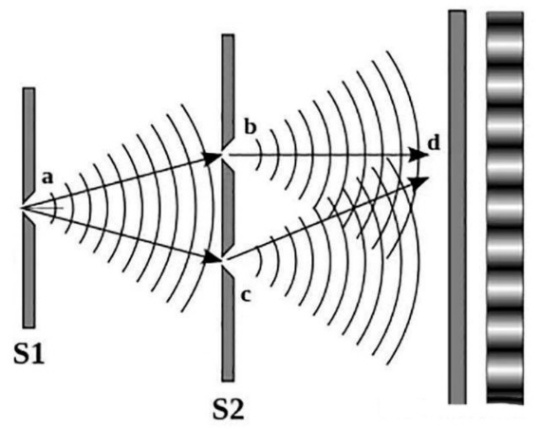
\includegraphics[width=\linewidth]{figures/图1.png}
        \caption{分波前法}
      \end{minipage}
      \hfill
      \begin{minipage}{0.33\textwidth}
        \centering
        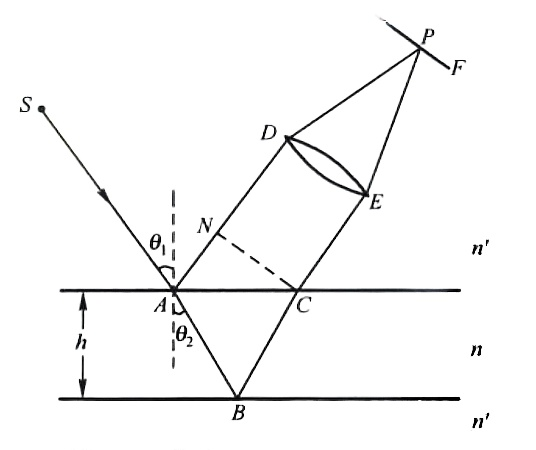
\includegraphics[width=\linewidth]{figures/图2.png}
        \caption{分振幅法}
      \end{minipage}
    \end{figure}

    \subsubsection{波长测量原理}
    双棱镜将同一狭缝发出的光分成两束，相当于两个相干虚光源。设虚光源间距为\(d\)，虚光源到观察屏的距离为\(D\)，
    屏上某点距条纹中心为\(x\)，在小角度近似下，光程差为
    \[
    \delta\approx\frac{dx}{D}
    \]
    
    相邻暗纹的光程差相差一个波长，因此条纹间距\(\Delta x\)满足
    \[
    \lambda=\frac{d\,\Delta x}{D}
    \]
    
    虚光源的位置和间距难以直接测量，实验中利用凸透镜二次成像法求得\(d\)和\(D\)，再测量\(\Delta x\)计算波长。

    \subsubsection{实验内容}
    \begin{enumerate}
      \item 光路调节：调节各元件等高共轴，依次调整透镜、狭缝、双棱镜和摄像头，使像与叉丝清晰可辨。
      \item 二次成像测量：在双棱镜与毛玻璃屏之间沿光轴移动透镜，找到分别形成放大像、缩小像的两个清晰位置，记录透镜位置及对应的像点间距，求出\(d\)和\(D\)。测量时，移动摄像头，使叉丝竖线对准像点中心；若像点过亮，可适当调小狭缝。
      \item 条纹间距测量：移开透镜，微调狭缝宽度，使干涉条纹与叉丝均清晰可辨。转动摄像头底座的螺旋测微器，对暗纹两侧明暗交界线分别读数，取平均值作为暗纹中心位置，据此求得条纹间距并计算波长。
    \end{enumerate}

  \subsection{实验重点（3分）}
  \begin{enumerate}
    \item 掌握分波面法干涉原理。
    \item 了解双棱镜干涉装置及光路调节技巧。
    \item 观察双棱镜干涉现象并测定光波波长。
  \end{enumerate}

  \subsection{实验难点（2分）}
  \begin{enumerate}
    \item 完成等高共轴调节，并通过狭缝宽度调节获得清晰条纹。
    \item 准确找到两个清晰成像位置，测量像点间距及相关距离。
    \item 准确定位暗纹中心，减小读数误差。
  \end{enumerate}

\section{实验操作与原始数据（50分）}
% 填写自己的实验数据图

\section{结果与分析（30分）}

  \subsection{数据处理与结果（20分）}  
  我们组先进行了二次成像法测$D$和$d$的实验，得到以下数据。
  其中我们先测的是最大清晰像的间距$d1$，然后再测最小清晰像的间距$d2$，
  两次测量的透镜位置分别为$v_{01}$和$v_{02}$，由此计算出物屏间距$D$。
  
  $\text{毛玻璃屏的位置}v_0 = 147.60\,\mathrm{cm}$，
  $\text{双棱镜位置} = 43.60\,\mathrm{cm}$，$\text{狭缝位置} = 21.60\,\mathrm{cm}$。

  \begin{figure}[H]
    \centering
    \begin{minipage}{0.4\textwidth}
      \centering
      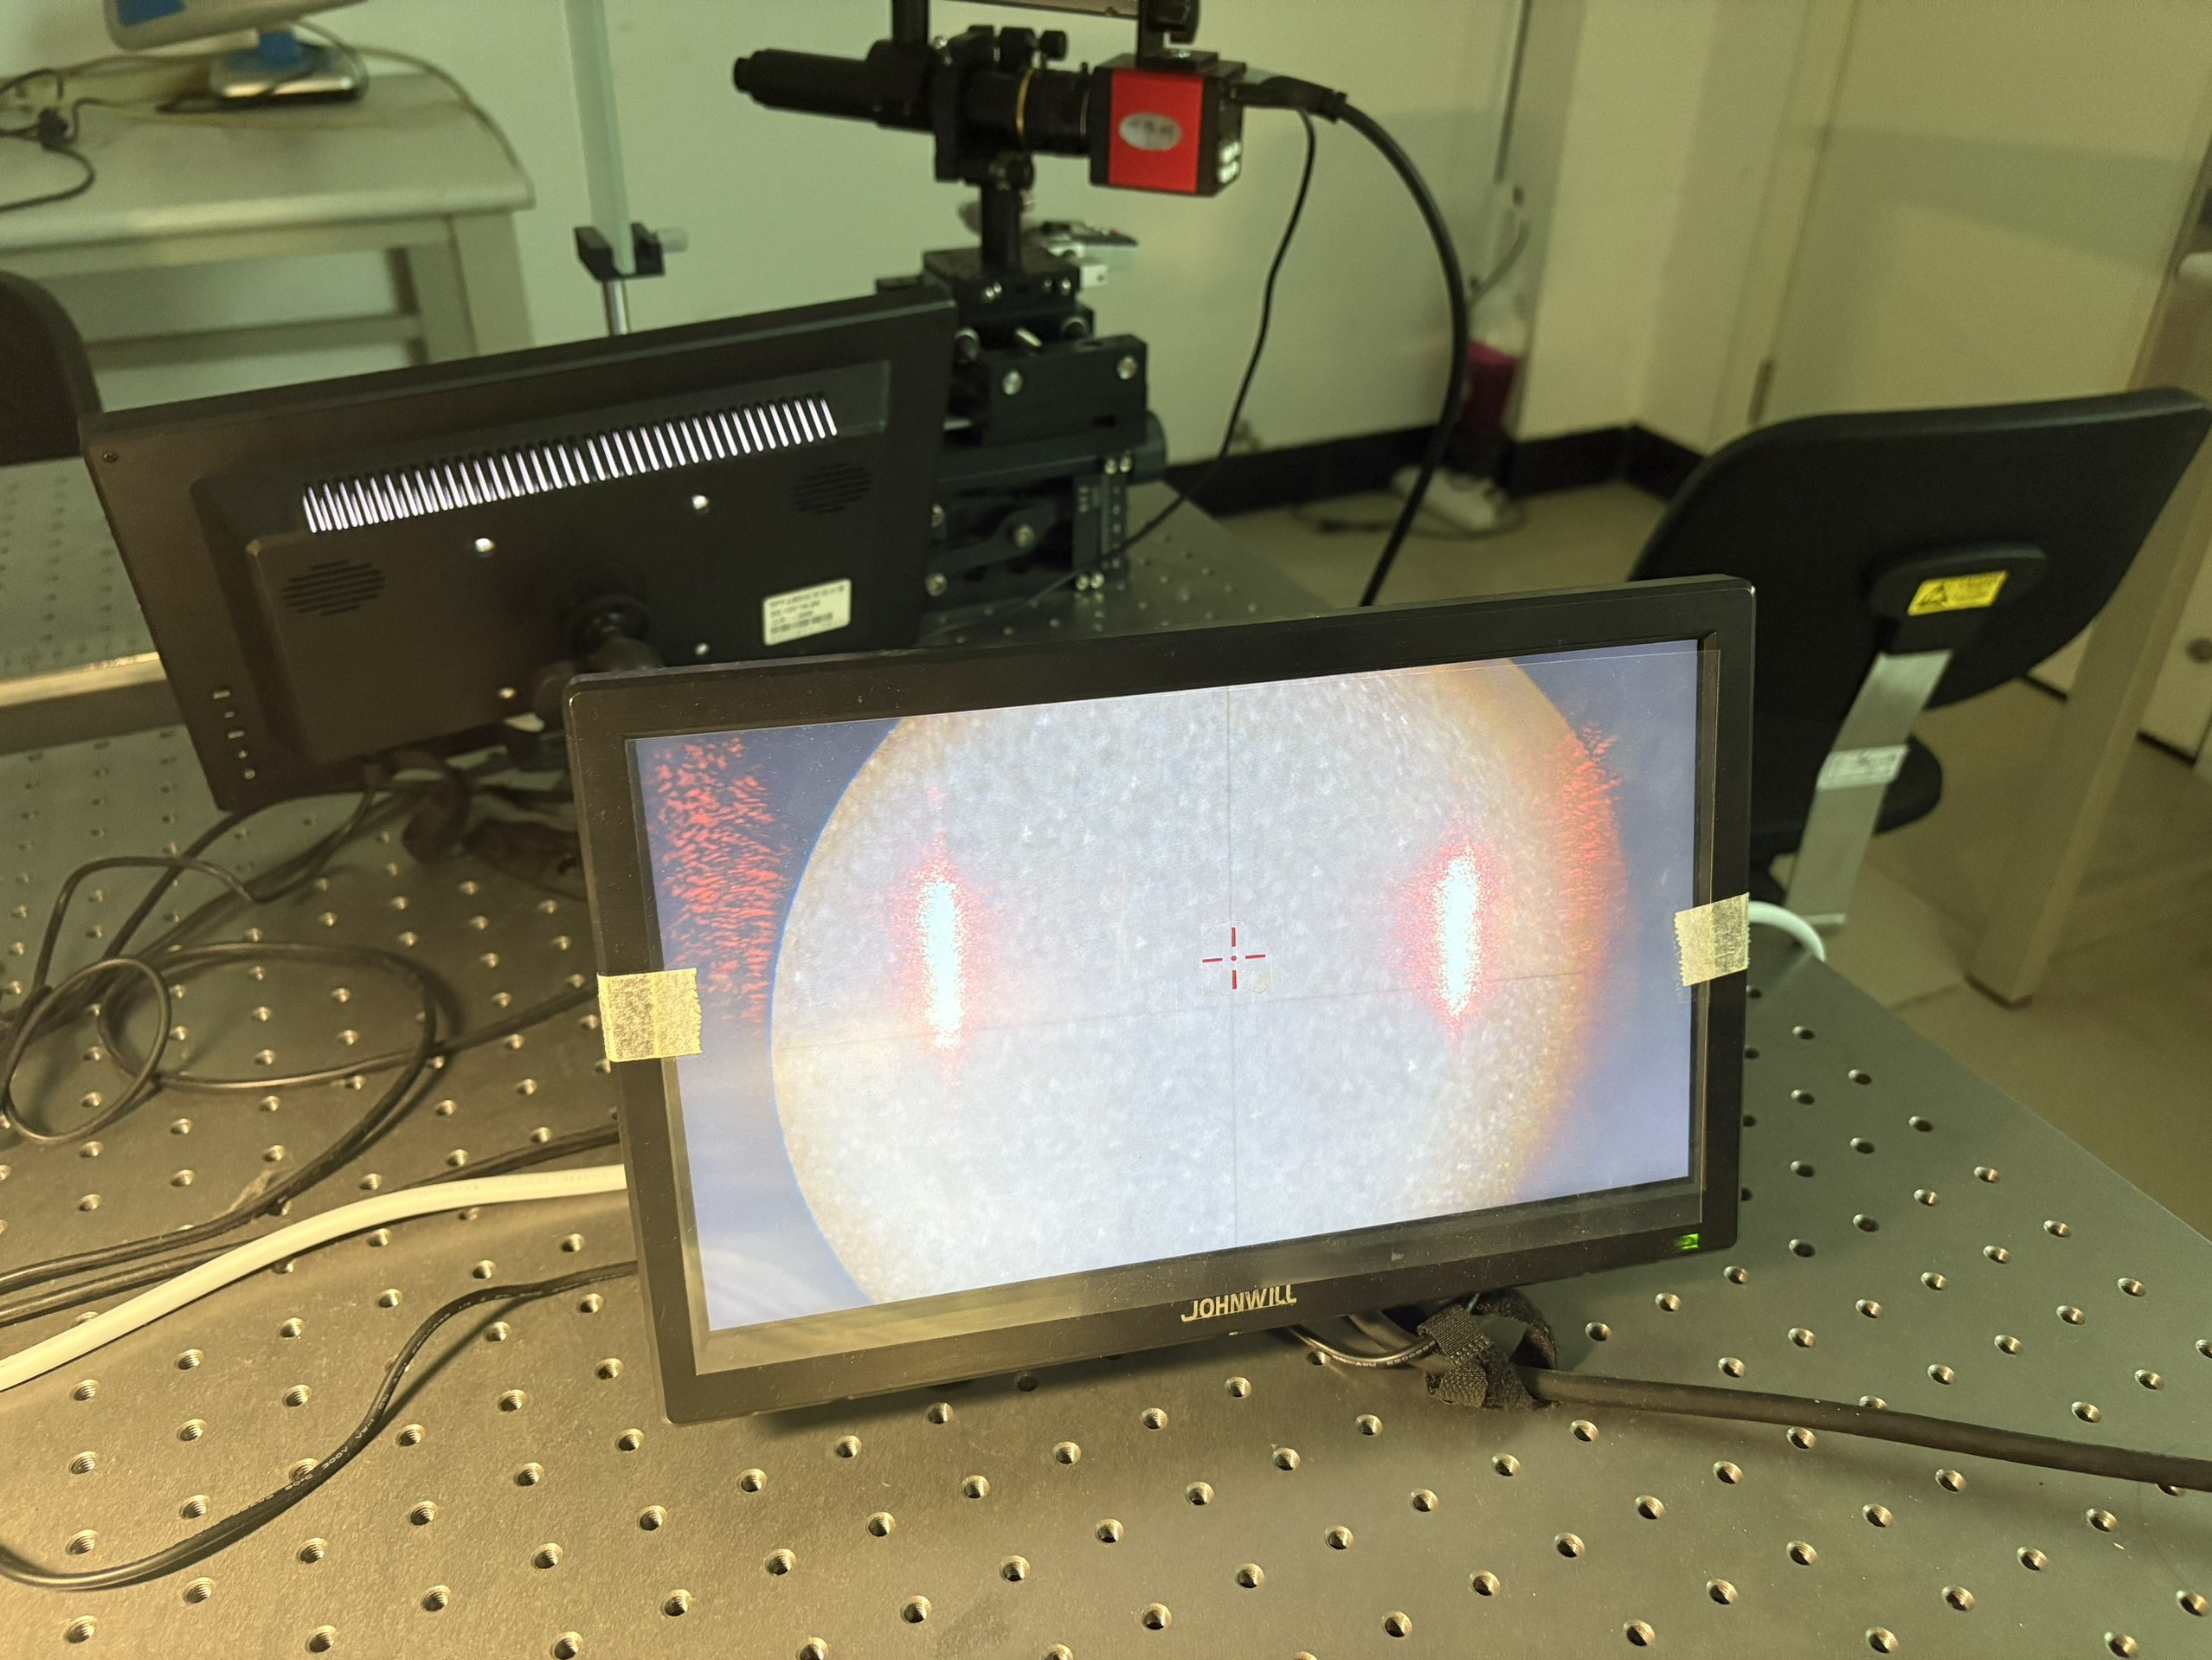
\includegraphics[width=\linewidth]{figures/图4.png}
      \caption{最大清晰像}
    \end{minipage}
    \hfill
    \begin{minipage}{0.4\textwidth}
      \centering
      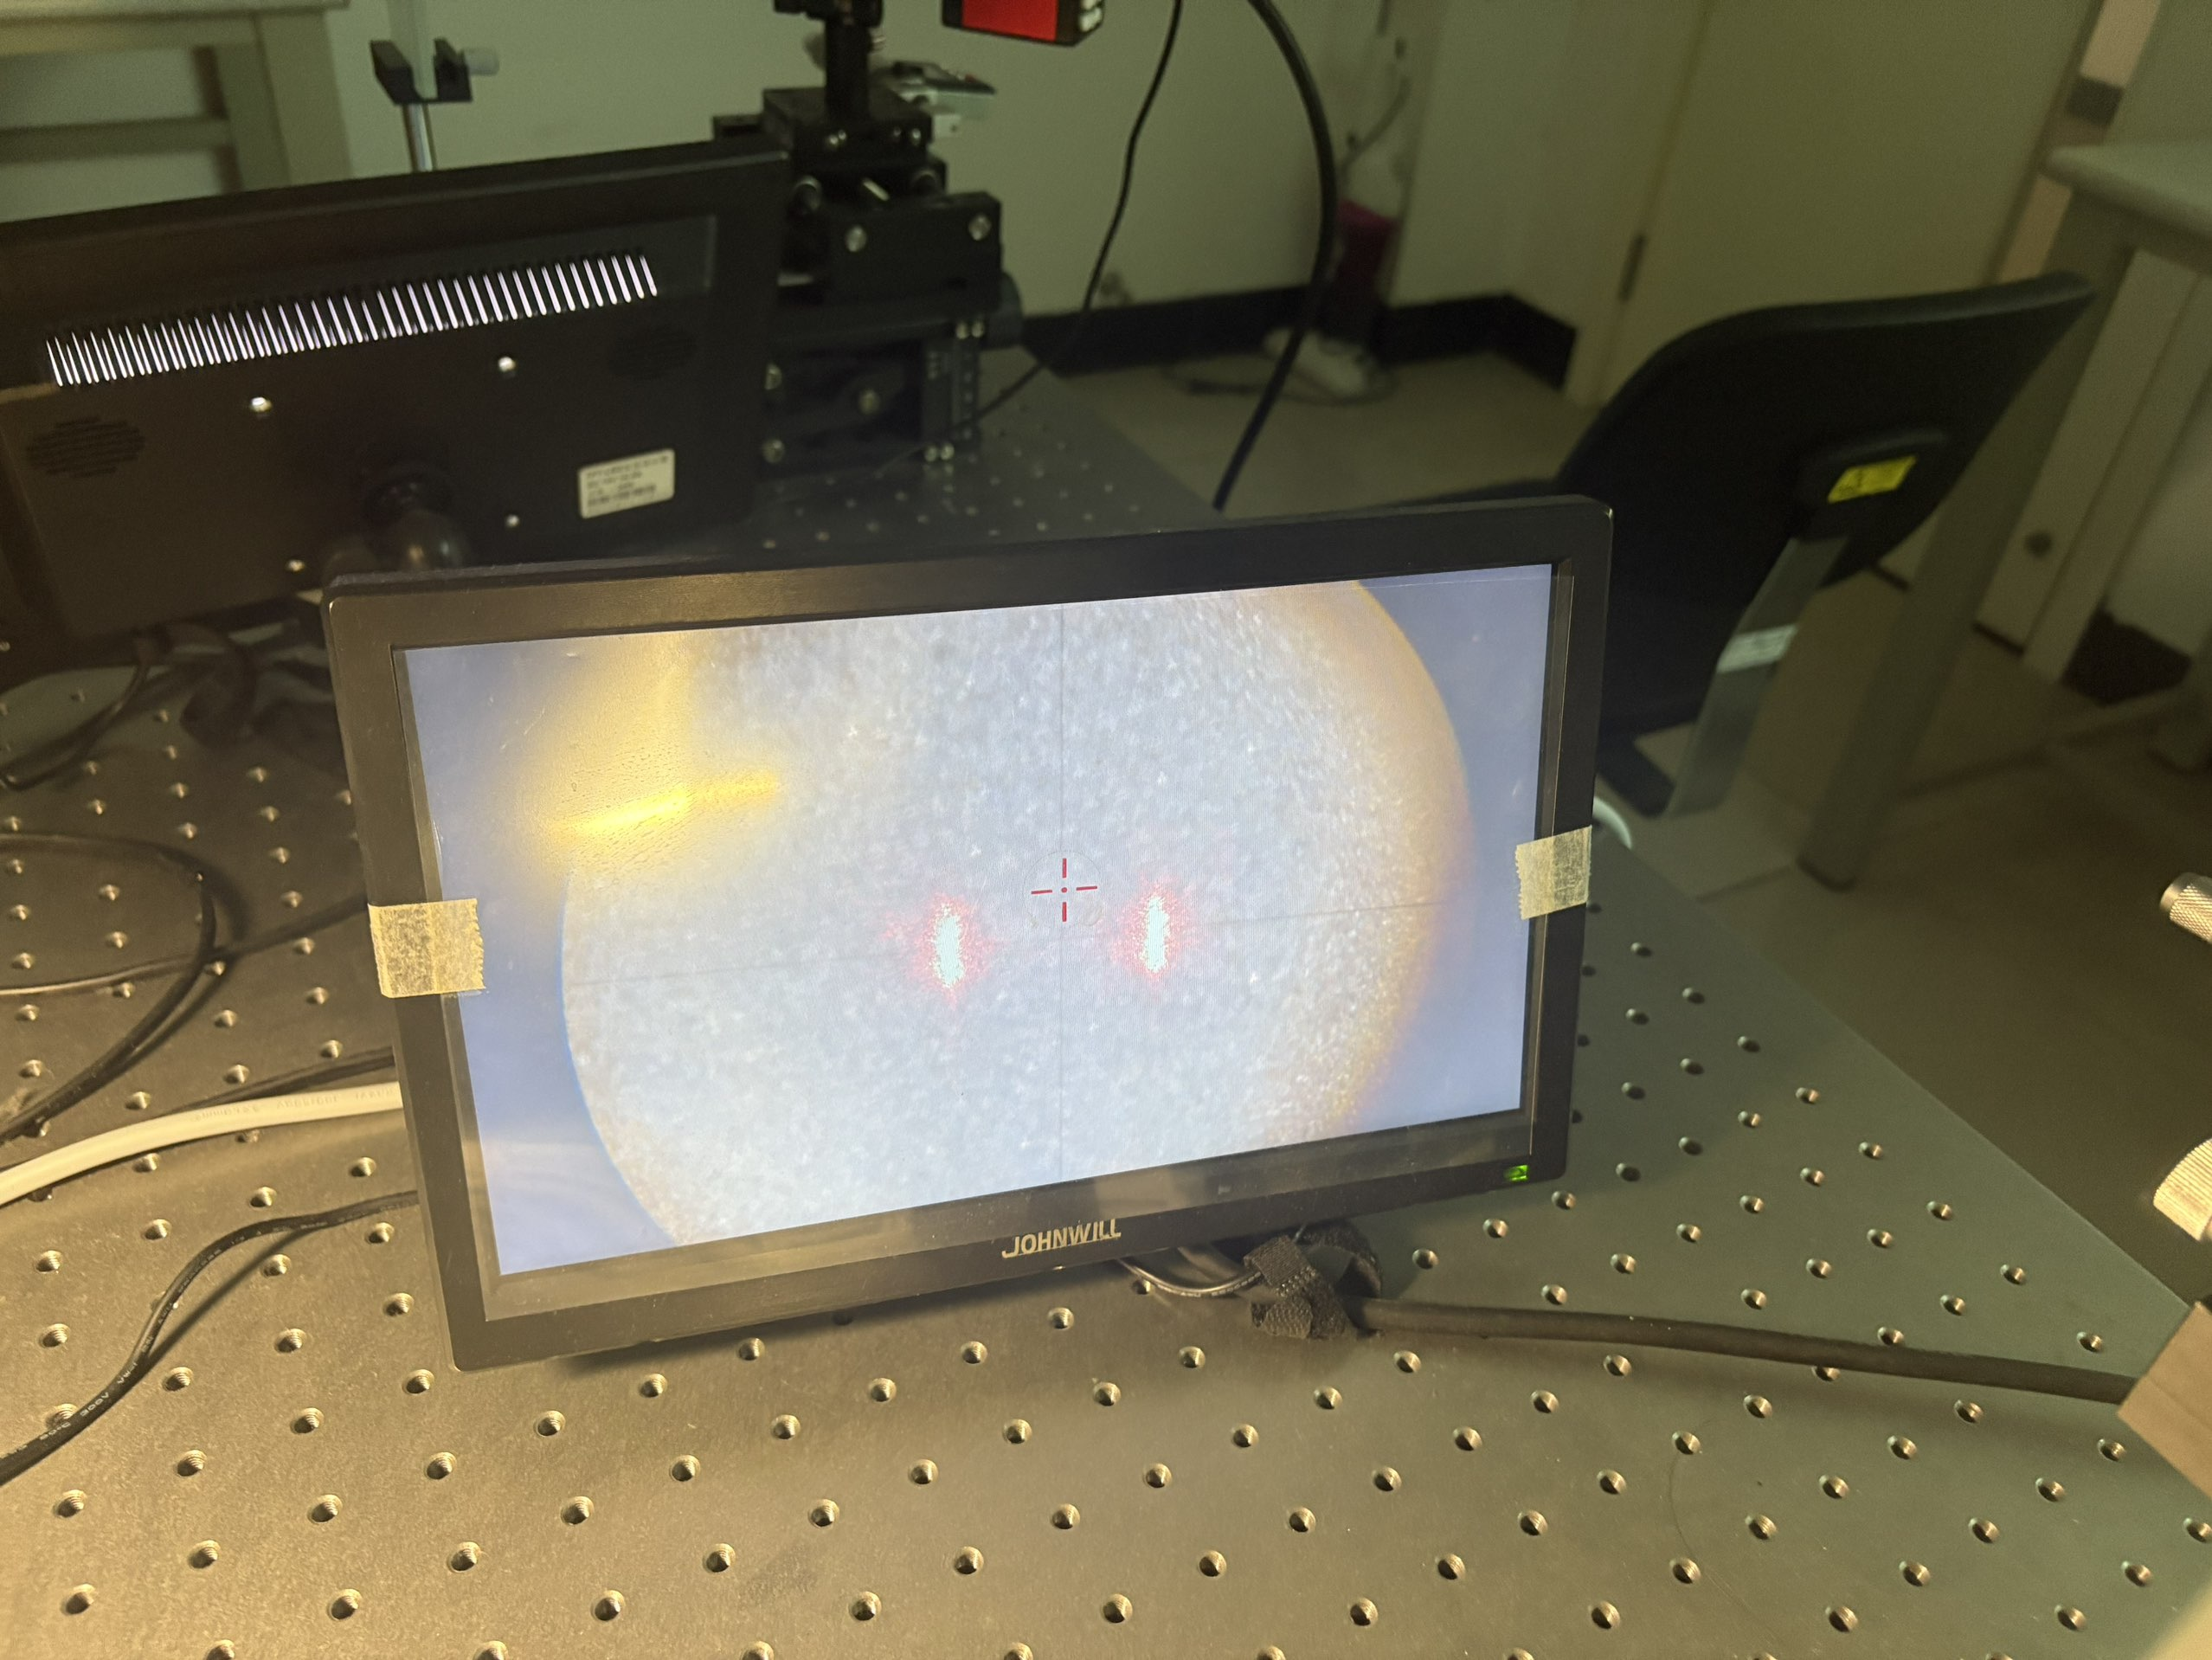
\includegraphics[width=\linewidth]{figures/图5.png}
      \caption{最小清晰像}
    \end{minipage}
  \end{figure}

  \begin{table}[H]
    \centering
    \caption{二次成像法测$D$和$d$}
    \begin{tabular}{cccccc}
      \toprule
      $\text{实验次数}$ & $v_{01}/\mathrm{cm}$ & $v_{02}/\mathrm{cm}$ & 
      $D/\mathrm{cm}$ & $d_1/\mathrm{mm}$ & $d_2/\mathrm{mm}$ \\
      \midrule
      1 & 69.58 & 97.79 & 127.83 & 4.241 & 1.667 \\
      2 & 69.65 & 97.76 & 127.79 & 4.268 & 1.695 \\
      3 & 69.53 & 97.75 & 127.92 & 4.282 & 1.674 \\
      4 & 69.59 & 97.69 & 127.92 & 4.192 & 1.628 \\
      5 & 69.55 & 97.74 & 127.91 & 4.195 & 1.655 \\
      6 & 69.60 & 97.79 & 127.81 & 4.248 & 1.670 \\
      \bottomrule
    \end{tabular}
  \end{table}

  由表中测量结果，分别计算$d_1$、$d_2$和$D$的平均值及平均值的A类标准不确定度。
  令$x$分别代表$d_1$、$d_2$或$D$，则
  \[
    \overline{x}=\frac{1}{6}\sum_{i=1}^{6}x_i,\qquad
    u_{\mathrm{A}}(\overline{x})=
    \sqrt{\frac{\sum_{i=1}^{6}(x_i-\overline{x})^2}{6\times5}}
  \]

  计算得到
  \[
    \begin{aligned}
      \overline{d}_1&=4.237667\,\mathrm{mm},
      &u_{\mathrm{A}}(\overline{d}_1)&=0.015176\,\mathrm{mm},\\
      \overline{d}_2&=1.664833\,\mathrm{mm},
      &u_{\mathrm{A}}(\overline{d}_2)&=0.009090\,\mathrm{mm},\\
      \overline{D}&=127.863333\,\mathrm{cm},
      &u_{\mathrm{A}}(\overline{D})&=0.024449\,\mathrm{cm}
    \end{aligned}
  \]

  光具座上的透镜位置和毛玻璃屏位置由直尺读出，像间距则由读数显微镜测量。已知
  \[
    \Delta_{\text{直尺}}=0.2\,\mathrm{mm}=0.02\,\mathrm{cm},\qquad
    \Delta_{\text{显微镜}}=0.004\,\mathrm{mm}
  \]

  仪器误差采用均匀分布模型，计算得到像间距的B类标准不确定度为
  \[
    u_{\mathrm{B}}(d_1)=u_{\mathrm{B}}(d_2)
      =\frac{0.004}{\sqrt{3}}\,\mathrm{mm}
      =0.002309\,\mathrm{mm}
  \]

  $D$由毛玻璃屏位置$v_0$及两个透镜位置$v_{01}$、$v_{02}$算得：
  \[
    D=(v_0-v_{01})+(v_0-v_{02})=2v_0-v_{01}-v_{02}
  \]
  
  则$D$的B类标准不确定度为
  \[
    u_{\mathrm{B}}(D)=\frac{\Delta_{\text{直尺}}}{\sqrt{3}}
       =\frac{0.02}{\sqrt{3}}\,\mathrm{cm}
       =0.011547\,\mathrm{cm}
  \]

  将A类和B类标准不确定度合成，得到
  \[
    \begin{aligned}
      u_{d_1}&=\sqrt{u_{\mathrm{A}}^2(\overline{d}_1)+u_{\mathrm{B}}^2(d_1)}
               =0.015351\,\mathrm{mm},\\
      u_{d_2}&=\sqrt{u_{\mathrm{A}}^2(\overline{d}_2)+u_{\mathrm{B}}^2(d_2)}
               =0.009379\,\mathrm{mm},\\
      u_D&=\sqrt{u_{\mathrm{A}}^2(\overline{D})+u_{\mathrm{B}}^2(D)}
               =0.027039\,\mathrm{cm}
    \end{aligned}
  \]

  不确定度保留两位有效数字，平均值保留至与不确定度末位相同的数位，得到结果为
  \[
    \begin{aligned}
      d_1&=\overline{d}_1\pm u_{d_1}
          =(4.238\pm0.015)\,\mathrm{mm},\\
      d_2&=\overline{d}_2\pm u_{d_2}
          =(1.6648\pm0.0094)\,\mathrm{mm},\\
      D&=\overline{D}\pm u_D
          =(127.863\pm0.027)\,\mathrm{cm}
    \end{aligned}
  \]

  完成上述实验后，我们组接着进行了用衍射法测波长的实验，得到以下暗纹位置数据。

  \begin{figure}[H]
    \centering
    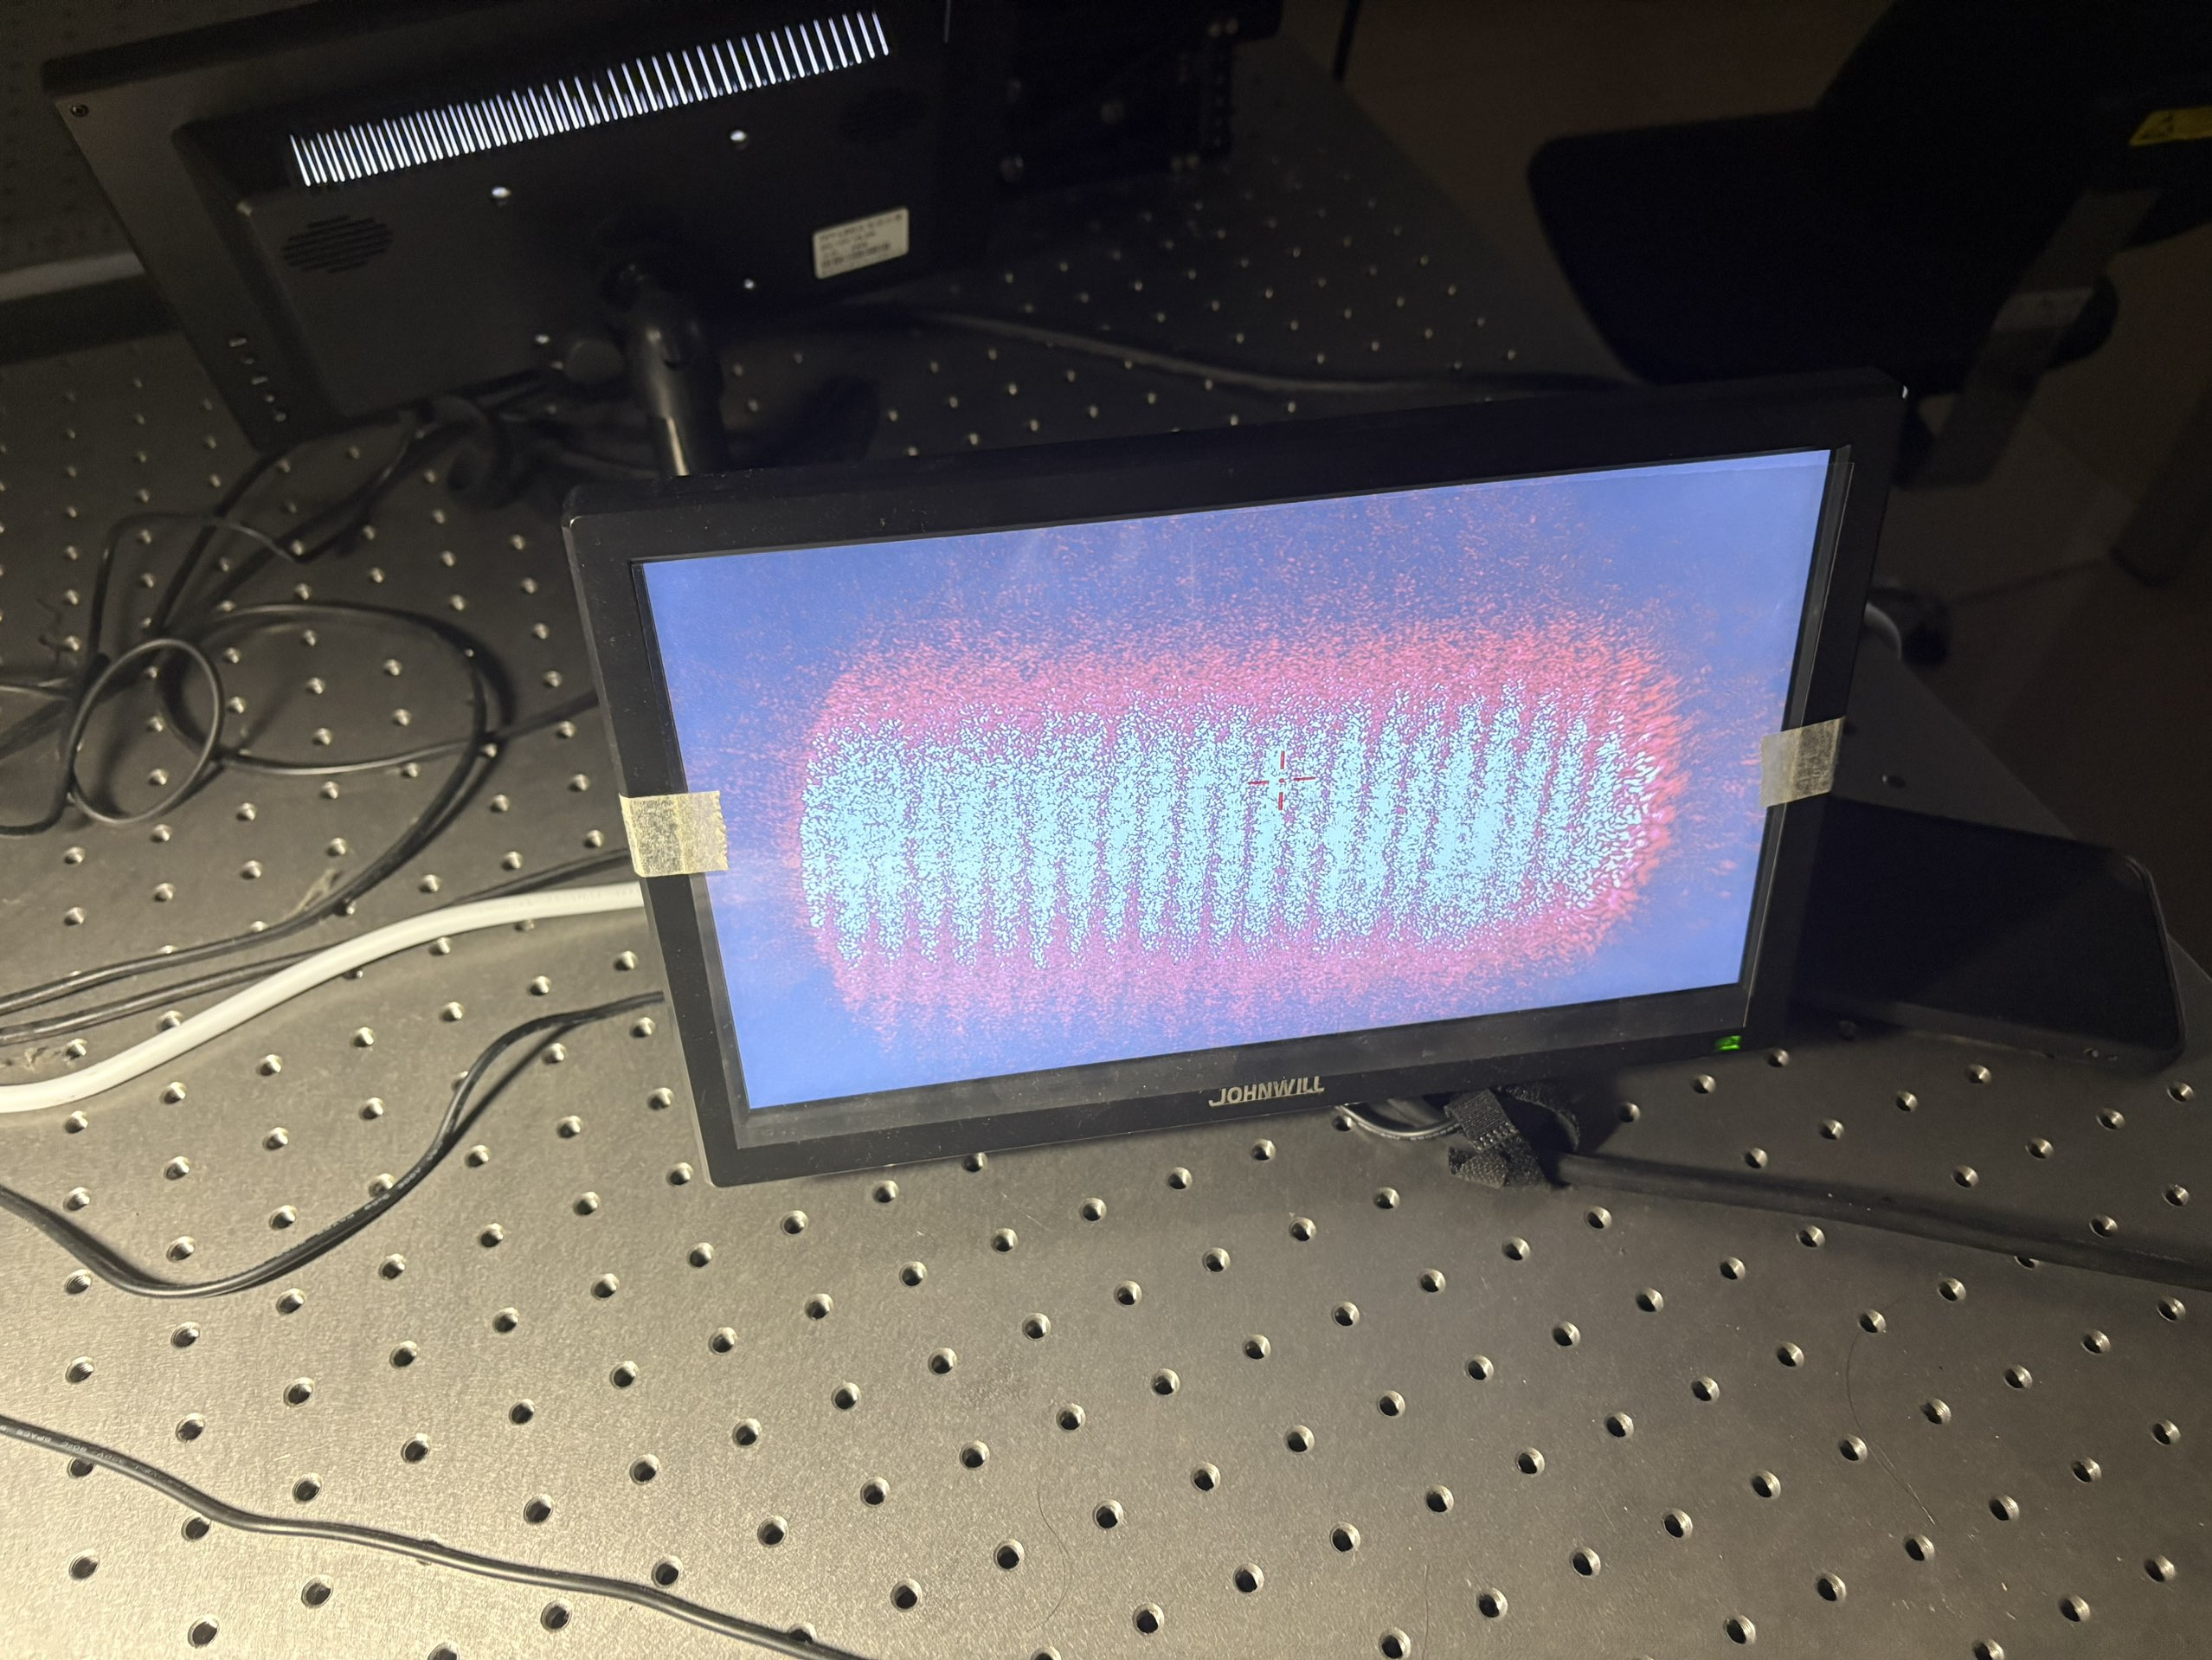
\includegraphics[width=0.5\textwidth]{figures/图6.png}    
    \caption{清晰衍射条纹}
  \end{figure}

  \begin{table}[H]
    \centering
    \caption{波长测量实验（读数单位：$\mathrm{mm}$）}
    \begin{tabular}{cccccccc}
      \toprule
      编号 & 左 & 右 & 平均$S_i$ & 编号 & 左 & 右 & 平均$S_i$ \\
      \midrule
      S1 & -0.053 & 0.091 & 0.019 & S11 & 2.947 & 3.033 & 2.990 \\
      S2 & 0.259 & 0.367 & 0.313 & S12 & 3.232 & 3.339 & 3.286 \\
      S3 & 0.531 & 0.641 & 0.586 & S13 & 3.561 & 3.650 & 3.606 \\
      S4 & 0.864 & 0.958 & 0.911 & S14 & 3.847 & 3.971 & 3.909 \\
      S5 & 1.142 & 1.256 & 1.199 & S15 & 4.138 & 4.252 & 4.195 \\
      S6 & 1.428 & 1.537 & 1.483 & S16 & 4.442 & 4.555 & 4.499 \\
      S7 & 1.724 & 1.835 & 1.780 & & & & \\
      S8 & 2.051 & 2.145 & 2.098 & & & & \\
      S9 & 2.334 & 2.419 & 2.377 & & & & \\
      S10 & 2.643 & 2.734 & 2.689 & & & & \\
      \bottomrule
    \end{tabular}
  \end{table}

  表中平均位置按$S_i=(S_{i,\mathrm{L}}+S_{i,\mathrm{R}})/2$计算，其中$\mathrm{L}$、$\mathrm{R}$分别表示左、右两侧读数；
  表内平均值按四舍五入保留三位小数。

  接下来我们进行数据处理。

  \noindent （1）逐差法求条纹间距
  由公式
  \[
    10\Delta x_i=S_{i+10}-S_i,\qquad i=1,2,\ldots,6
  \]
  直接采用表中已四舍五入保留三位小数的平均位置$S_i$，得到六组逐差结果为
  \[
    \begin{aligned}
      10\Delta x_1&=2.990-0.019=2.971\,\mathrm{mm},10\Delta x_2&=3.286-0.313=2.973\,\mathrm{mm},\\
      10\Delta x_3&=3.606-0.586=3.020\,\mathrm{mm},10\Delta x_4&=3.909-0.911=2.998\,\mathrm{mm},\\
      10\Delta x_5&=4.195-1.199=2.996\,\mathrm{mm},10\Delta x_6&=4.499-1.483=3.016\,\mathrm{mm}
    \end{aligned}
  \]

  除以$10$，得到六组条纹间距
  \[
    (\Delta x_1,\ldots,\Delta x_6)
    =(0.297100,\ 0.297300,\ 0.302000,\ 0.299800,\ 0.299600,\ 0.301600)\,\mathrm{mm}
  \]

  \noindent （2）条纹间距的估计值及不确定度

  将六组逐差所得间距视为同一条纹间距的等精度测量值，作等权最小二乘估计。令待估间距为$q$，使
  \[
    Q(q)=\sum_{i=1}^{6}(\Delta x_i-q)^2
  \]
  最小，即使得$\mathrm{d}Q/\mathrm{d}q=0$，得到最小二乘估计即六组间距的算术平均值：
  \[
    \overline{\Delta x}=\frac{1}{6}\sum_{i=1}^{6}\Delta x_i
      =\frac{1}{60}\sum_{i=1}^{6}(S_{i+10}-S_i)
      =0.299567\,\mathrm{mm}
  \]

  所以平均间距的A类标准不确定度为
  \[
    u_{\mathrm{A}}(\overline{\Delta x})
      =\sqrt{\frac{\sum_{i=1}^{6}(\Delta x_i-\overline{\Delta x})^2}{6\times5}}
      =0.000843\,\mathrm{mm}
  \]

  B类分量为
  \[
    u_{\mathrm{B}}(\Delta x)
      =\frac{0.004}{\sqrt{3}}\,\mathrm{mm}
      =0.002309\,\mathrm{mm}
  \]

  合成标准不确定度为
  \[
    u_{\Delta x}
      =\sqrt{u_{\mathrm{A}}^2(\overline{\Delta x})+u_{\mathrm{B}}^2(\Delta x)}
      =0.002459\,\mathrm{mm}
  \]

  同样的，不确定度保留两位有效数字，条纹间距的结果写为
  \[
    \boxed{\Delta x=\overline{\Delta x}\pm u_{\Delta x}
      =(0.2996\pm0.0025)\,\mathrm{mm}}
  \]

  \noindent （3）波长及其不确定度

  利用二次成像法得到的虚光源间距$d=\sqrt{\overline{d}_1\,\overline{d}_2}$，波长为
  \[
    \overline{\lambda}
      =\frac{\sqrt{\overline{d}_1\,\overline{d}_2}}{\overline{D}}\,
        \overline{\Delta x}
  \]

  将已知结果$\overline{D}=127.863\,\mathrm{cm}=1278.63\,\mathrm{mm}$、$\overline{d}_1=4.238\,\mathrm{mm}$、$\overline{d}_2=1.6648\,\mathrm{mm}$及$\overline{\Delta x}=0.2996\,\mathrm{mm}$代入，计算得
  \[
    \overline{\lambda}
      =\frac{\sqrt{4.238\times1.6648}}{1278.63}
        \times0.2996\,\mathrm{mm}
      \approx0.000622384\,\mathrm{mm}
      =622.384\,\mathrm{nm}
  \]

  按所给不确定度传播公式，有
  \[
    \frac{u_\lambda}{\overline{\lambda}}
      =\sqrt{\left(\frac{u_{d_1}}{2\overline{d}_1}\right)^2
             +\left(\frac{u_{d_2}}{2\overline{d}_2}\right)^2
             +\left(\frac{u_{\Delta x}}{\overline{\Delta x}}\right)^2
             +\left(\frac{u_D}{\overline{D}}\right)^2}
  \]

  代入前述测量结果，即$u_{d_1}=0.015\,\mathrm{mm}$、$u_{d_2}=0.0094\,\mathrm{mm}$、$u_{\Delta x}=0.0025\,\mathrm{mm}$和$u_D=0.027\,\mathrm{cm}$，得
  \[
    \begin{aligned}
      \frac{u_\lambda}{\overline{\lambda}}
        &=\sqrt{(0.0017697)^2+(0.0028232)^2
                 +(0.0083445)^2+(0.0002112)^2}\\
        &=0.0089876\approx0.899\%,\\
      u_\lambda&=622.384\times0.0089876\,\mathrm{nm}
                 =5.594\,\mathrm{nm}
    \end{aligned}
  \]

  最终波长测量结果为
  \[
    \boxed{\lambda=\overline{\lambda}\pm u_\lambda
      =(622.384\pm5.594)\,\mathrm{nm}}
  \]

  \subsection{误差分析（10分）}
  本实验的误差主要来自以下几个方面：
  \begin{enumerate}
    \item 条纹位置的判断：条纹模糊或对焦不准时，暗纹边界与叉丝难以准确对齐，影响条纹间距$\Delta x$的测量。
    该项相对不确定度较大，是波长不确定度的主要来源。

    \item 二次成像的判断：放大像和缩小像未调至最清晰时，
    透镜位置及像间距$d_1$、$d_2$的读数会产生偏差，进而影响虚光源间距$d$的计算。

    \item 光路调节：各元件未等高共轴，会使成像质量下降；条纹倾斜时，沿测量方向读出的间距偏大，使计算得到的波长偏大。
    
    \item 仪器与环境影响：仪器精度、读数视差及显微镜的回程间隙均会引入误差，振动和气流也会使条纹抖动。
    应尽量单向移动显微镜，待条纹稳定后读数。
  \end{enumerate}

\section{实验探讨与思考题（10分）}

  \subsection{实验探讨}
  本次实验中，我体会最深的是仪器调节的重要性。
  各元件应等高共轴，保证透镜移动到两个成像位置时光路都畅通。摄像头要调好位置并准确对焦，使条纹和叉丝清晰，便于读数。
  二次成像时，应仔细微调透镜，找到最清晰的放大像和缩小像后再记录数据。

  \subsection{思考题}

    \subsubsection{为减小测量误差，应该如何设置狭缝到屏的距离D，狭缝到双棱镜的距离？}
    在条纹清晰、两束光的重叠区域足够大且光具座长度允许的条件下，应适当增大狭缝到屏的距离$D$，并适当减小狭缝到双棱镜的距离$a$。
    由
    \[
      \Delta x=\frac{\lambda D}{d}
    \]
    可知，增大$D$可增大条纹间距。
    对于给定双棱镜，虚光源间距$d$与狭缝到双棱镜的距离$a$近似成正比，因此减小$a$也能增大条纹间距。
    在读数绝对误差近似不变时，这有助于减小条纹间距的相对测量误差。

    距离选择还须兼顾条纹亮度、可见条纹数量及二次成像条件，满足$D>4f$，且两个清晰成像位置均应位于透镜的可移动范围内。

    \subsubsection{测量时如果条纹有倾斜，对测量结果有何影响？}
    测量条纹间距时，摄像头的移动方向应与条纹垂直。
    如果条纹倾斜，测量方向与条纹法线之间存在夹角$\theta$，沿测量方向读出的相邻条纹间距为
    \[
      \Delta x_{\text{测}}=\frac{\Delta x}{\cos\theta}
    \]
    
    因此，将该读数直接代入$\lambda=d\,\Delta x/D$会使波长测量值偏大，形成系统误差。
    若其他量准确，则相对偏差为
    \[
      \frac{\lambda_{\text{测}}-\lambda}{\lambda}
      =\frac{1}{\cos\theta}-1
    \]

    此外，条纹倾斜时，条纹与竖直叉丝难以重合，也会增加对准和读数的困难。
    测量前应调整狭缝和双棱镜等元件的方向，使干涉条纹与竖直叉丝平行，并保证横向测量方向与条纹垂直。

\vspace*{\fill} % 使下面内容在页面底部显示
\noindent
\begin{minipage}{\textwidth}
  注意事项：

  \begingroup
    \setlength{\leftskip}{2em} % 1--4整体向右缩进两个汉字宽度
    1. 用PDF格式上传“实验报告”，文件名：学生姓名+学号+实验名称+周次。

    2. “实验报告”必须递交在“学在浙大”本课程内对应实验项目的“作业”模块内。

    3. “实验报告”成绩必须在“浙江大学物理实验教学中心网站”-“选课系统”内查询。

    4. 教学评价必须在“浙江大学物理实验教学中心网站”-“选课系统”内进行，学生必须进行教学评价，才能看到实验报告成绩，教学评价须在本次实验结束之后3天内进行。\par
  \endgroup

  \begin{center}
    {\CJKfontspec[AutoFakeBold=2.5]{SimSun}\bfseries 浙江大学物理实验教学中心制}
  \end{center}
\end{minipage}

\end{document}
